\documentclass[11pt, fleqn]{article}
\usepackage{../../../../template/template}

%сам документ
\begin{document}
    \begin{center}
      \huge ДЗ по алгебре №2, 3 сем

      \Large (преподаватель Демченко О. В.)

      \large Записал Костин П.А.

      \tableofcontents
    	\newpage
    \end{center}

    \section{Формулировка задания}
    \begin{task}
        $G$ - группа порядка 24
        \begin{enumerate}
          \item Найти все подгруппы $G$ порядка 3 и 4.
          \item Выбрать одну из ненормальных подгрупп порядка 3 (если они есть) и выписать задаваемое ей разбиение $G$ на левые и правые классы смежности.

          В случае, если все подгруппы $G$ порядка 3 являются нормальными, найти нормальную подгруппу порядка 4 и выписать задаваемое ей разбиение $G$ на левые и правые классы смежности.
          \item Выбрать одну из нормальных подгрупп $G$ порядка 3 (если они есть),
          построить таблицу Кэли для соответствующей факторгруппы и определить, какой из перечисленных в приложении групп порядка 8 она
          изоморфна.

          В случае, если все подгруппы $G$ порядка 3 являются ненормальными,
          найти нормальную подгруппу порядка 2, построить таблицу Кэли для
          соответствующей факторгруппы и определить, какой из перечисленных в приложении групп порядка 12 она изоморфна.

          В случае, если все подгруппы $G$ порядка 2 и 3 являются ненормальными, найти нормальную подгруппу порядка 4 и построить таблицу Кэли для соответствующей факторгруппы. Кроме того, в этом случае необходимо выбрать произвольную подгруппу G порядка 8 и определить, какой из перечисленных в приложении групп она изоморфна.
          \item Описать явно изоморфизм между соответствующими группами из предыдущего пункта и доказать, что это изоморфизм. (В случае представления совпадающий таблиц Кэли необходимо продемонстрировать, каким образом происходил поиск соответствующего упорядочивания).
          \item Есть ли изоморфная $G$ группа среди трех следующих за ней по списку?
          \item Найти коммутант $G$.
        \end{enumerate}
    \end{task}

    \begin{remark}[приложение]
        Группы порядка 8: $\Z_8,\ \Z_4 \times \Z_2,\ \Z_2 times \Z_2 \times \Z_2,\ D_4$, группа кватернионов $Q_8= \{\pm 1, \pm i, \pm j, \pm k\}$ с операцией $i^2 = j^2 = k^2 = -1,\ ij = -ji = k,\ jk = kj = i,\ ki = -ik = j$

        Группы порядка 12: $\Z_{12},\ \Z_2 \times \Z_6,\ D_6,\ A4,\ T = \Z_3 \times \Z_4$ с операцией $(b1, c1)(b2, c2) = (b1 + (-1)^{c1} b2, c1 + c2)$
    \end{remark}

    \begin{Remark}[мои данные]
        \[G = \SL_2(\Z_4)\setminus K,\q K = \{E_2,\ -E_2\}\]
        (можно считать, что $G$ состоит из матриц $A \in \SL_2(\Z_4)$) таких, что либо $a_{11} = \ol{1}$, либо $a_{11} = \ol{0}, \ol{2}$ и $a_{12} = \ol{1}$)
    \end{Remark}

    \section{Решение задачи}
    \begin{sol}
        Элементы моей группы и их порядки (сколько раз возводим в степень до получения единичной):
        \[\ 1. \begin{pmatrix}
            1 & 0\\
            0 & 1
        \end{pmatrix} - \textcolor{red}{1} \qq\ \
        2. \begin{pmatrix}
            0 & 1\\
            3 & 1
        \end{pmatrix} - \textcolor{red}{3} \qq\ \
        3.\begin{pmatrix}
            1 & 3\\
            1 & 0
        \end{pmatrix} - \textcolor{red}{3} \qq\ \
        4.\begin{pmatrix}
            0 & 1\\
            3 & 3
        \end{pmatrix} - \textcolor{red}{3}\]
        \[\ 5.\begin{pmatrix}
            1 & 1\\
            3 & 0
        \end{pmatrix} - \textcolor{red}{3} \qq\ \
        6.\begin{pmatrix}
            1 & 1\\
            1 & 2
        \end{pmatrix} - \textcolor{red}{3} \qq\ \
        7.\begin{pmatrix}
            2 & 1\\
            1 & 3
        \end{pmatrix} - \textcolor{red}{3} \qq\ \
        8.\begin{pmatrix}
            1 & 3\\
            3 & 2
        \end{pmatrix} - \textcolor{red}{3}\]
        \[\ 9.\begin{pmatrix}
            2 & 1\\
            1 & 1
        \end{pmatrix} - \textcolor{red}{3} \qq\
        10.\begin{pmatrix}
            0 & 1\\
            3 & 0
        \end{pmatrix} - \textcolor{red}{2} \qq
        11.\begin{pmatrix}
            1 & 0\\
            2 & 1
        \end{pmatrix} - \textcolor{red}{2} \qq
        12.\begin{pmatrix}
            1 & 1\\
            2 & 3
        \end{pmatrix} - \textcolor{red}{2}\]
        \[13.\begin{pmatrix}
            1 & 2\\
            0 & 1
        \end{pmatrix} - \textcolor{red}{2} \qq
        14.\begin{pmatrix}
            1 & 2\\
            1 & 3
        \end{pmatrix} - \textcolor{red}{2} \qq
        15.\begin{pmatrix}
            1 & 2\\
            2 & 1
        \end{pmatrix} - \textcolor{red}{2} \qq
        16.\begin{pmatrix}
            1 & 2\\
            3 & 3
        \end{pmatrix} - \textcolor{red}{2}\]
        \[17.\begin{pmatrix}
            2 & 1\\
            3 & 2
        \end{pmatrix} - \textcolor{red}{2} \qq
        18.\begin{pmatrix}
            1 & 3\\
            2 & 3
        \end{pmatrix} - \textcolor{red}{2} \qq
        19.\begin{pmatrix}
            0 & 1\\
            3 & 2
        \end{pmatrix} - \textcolor{red}{4} \qq
        20.\begin{pmatrix}
            1 & 0\\
            1 & 1
        \end{pmatrix} - \textcolor{red}{4}\]
        \[21.\begin{pmatrix}
            1 & 0\\
            3 & 1
        \end{pmatrix} - \textcolor{red}{4} \qq
        22.\begin{pmatrix}
            1 & 1\\
            0 & 1
        \end{pmatrix} - \textcolor{red}{4} \qq
        23.\begin{pmatrix}
            1 & 3\\
            0 & 1
        \end{pmatrix} - \textcolor{red}{4} \qq
        24.\begin{pmatrix}
            2 & 1\\
            3 & 0
        \end{pmatrix} - \textcolor{red}{4}\]
    \end{sol}

    \begin{enumerate}
      \subsection{Первый пункт}
      \subsubsection{Формулировка}
      \item Найти все подгруппы $G$ порядка 3 и 4.
      \subsubsection{Вспомогательные факты}

      \begin{theorem}[Лагранжа]
          $H < G$, $|G| < \infty$, тогда $|G| \devides |H|$
      \end{theorem}

      \begin{consequence}
          $|G| = p \RA$группа цикоическая
      \end{consequence}

      \begin{Utv}
        \[|H| = 4 \RA \left[ \begin{matrix}
            H \cong \Z_4 \text{ цикл}\\
            H \cong \Z_2 \times \Z_2
        \end{matrix}\right.\]
      \end{Utv}

      \begin{proof}
          В группе порядка 4 элементы имеют порядок 1, 2 или 4 (теорема Лагранжа)

          Нейтральный есть всегда, тогда нам нужно найти 3 другие элемента

          Предположим, что элементов порядка 4 хотя бы два, тогда необходимо, чтобы $a^2=a^3 \neq e$ лежал там, а это невозможно. Значит элементов порядка 4 не больше одного

          Если элемент порядка 4 один, тогда в этой группе лежат $a,\ a^2,\ a^3$ и $e$

          Других вариантов нет для этого случая

          Тогда остался случай с нейтральным и 3 элементами порядка 2: e, a, b, c

          Нужно, чтобы все произведения лежали в группе

          Тогда $ab=ba=c\ ac=ca=b\ bc=cb=a$
      \end{proof}

      \subsubsection{Решение}
      Знаем, что если $H < G$, $H=3$ - простое $\Ra$ $H$ - циклическая (может быть порождена одним элементом a, то есть все её элементы являются степенями a).

      Порядок подгрупп должен делиться на порядок входящих в неё элементов (следствие из теоремы Лагранжа)\\
      \begin{figure}[h]
          \centering
          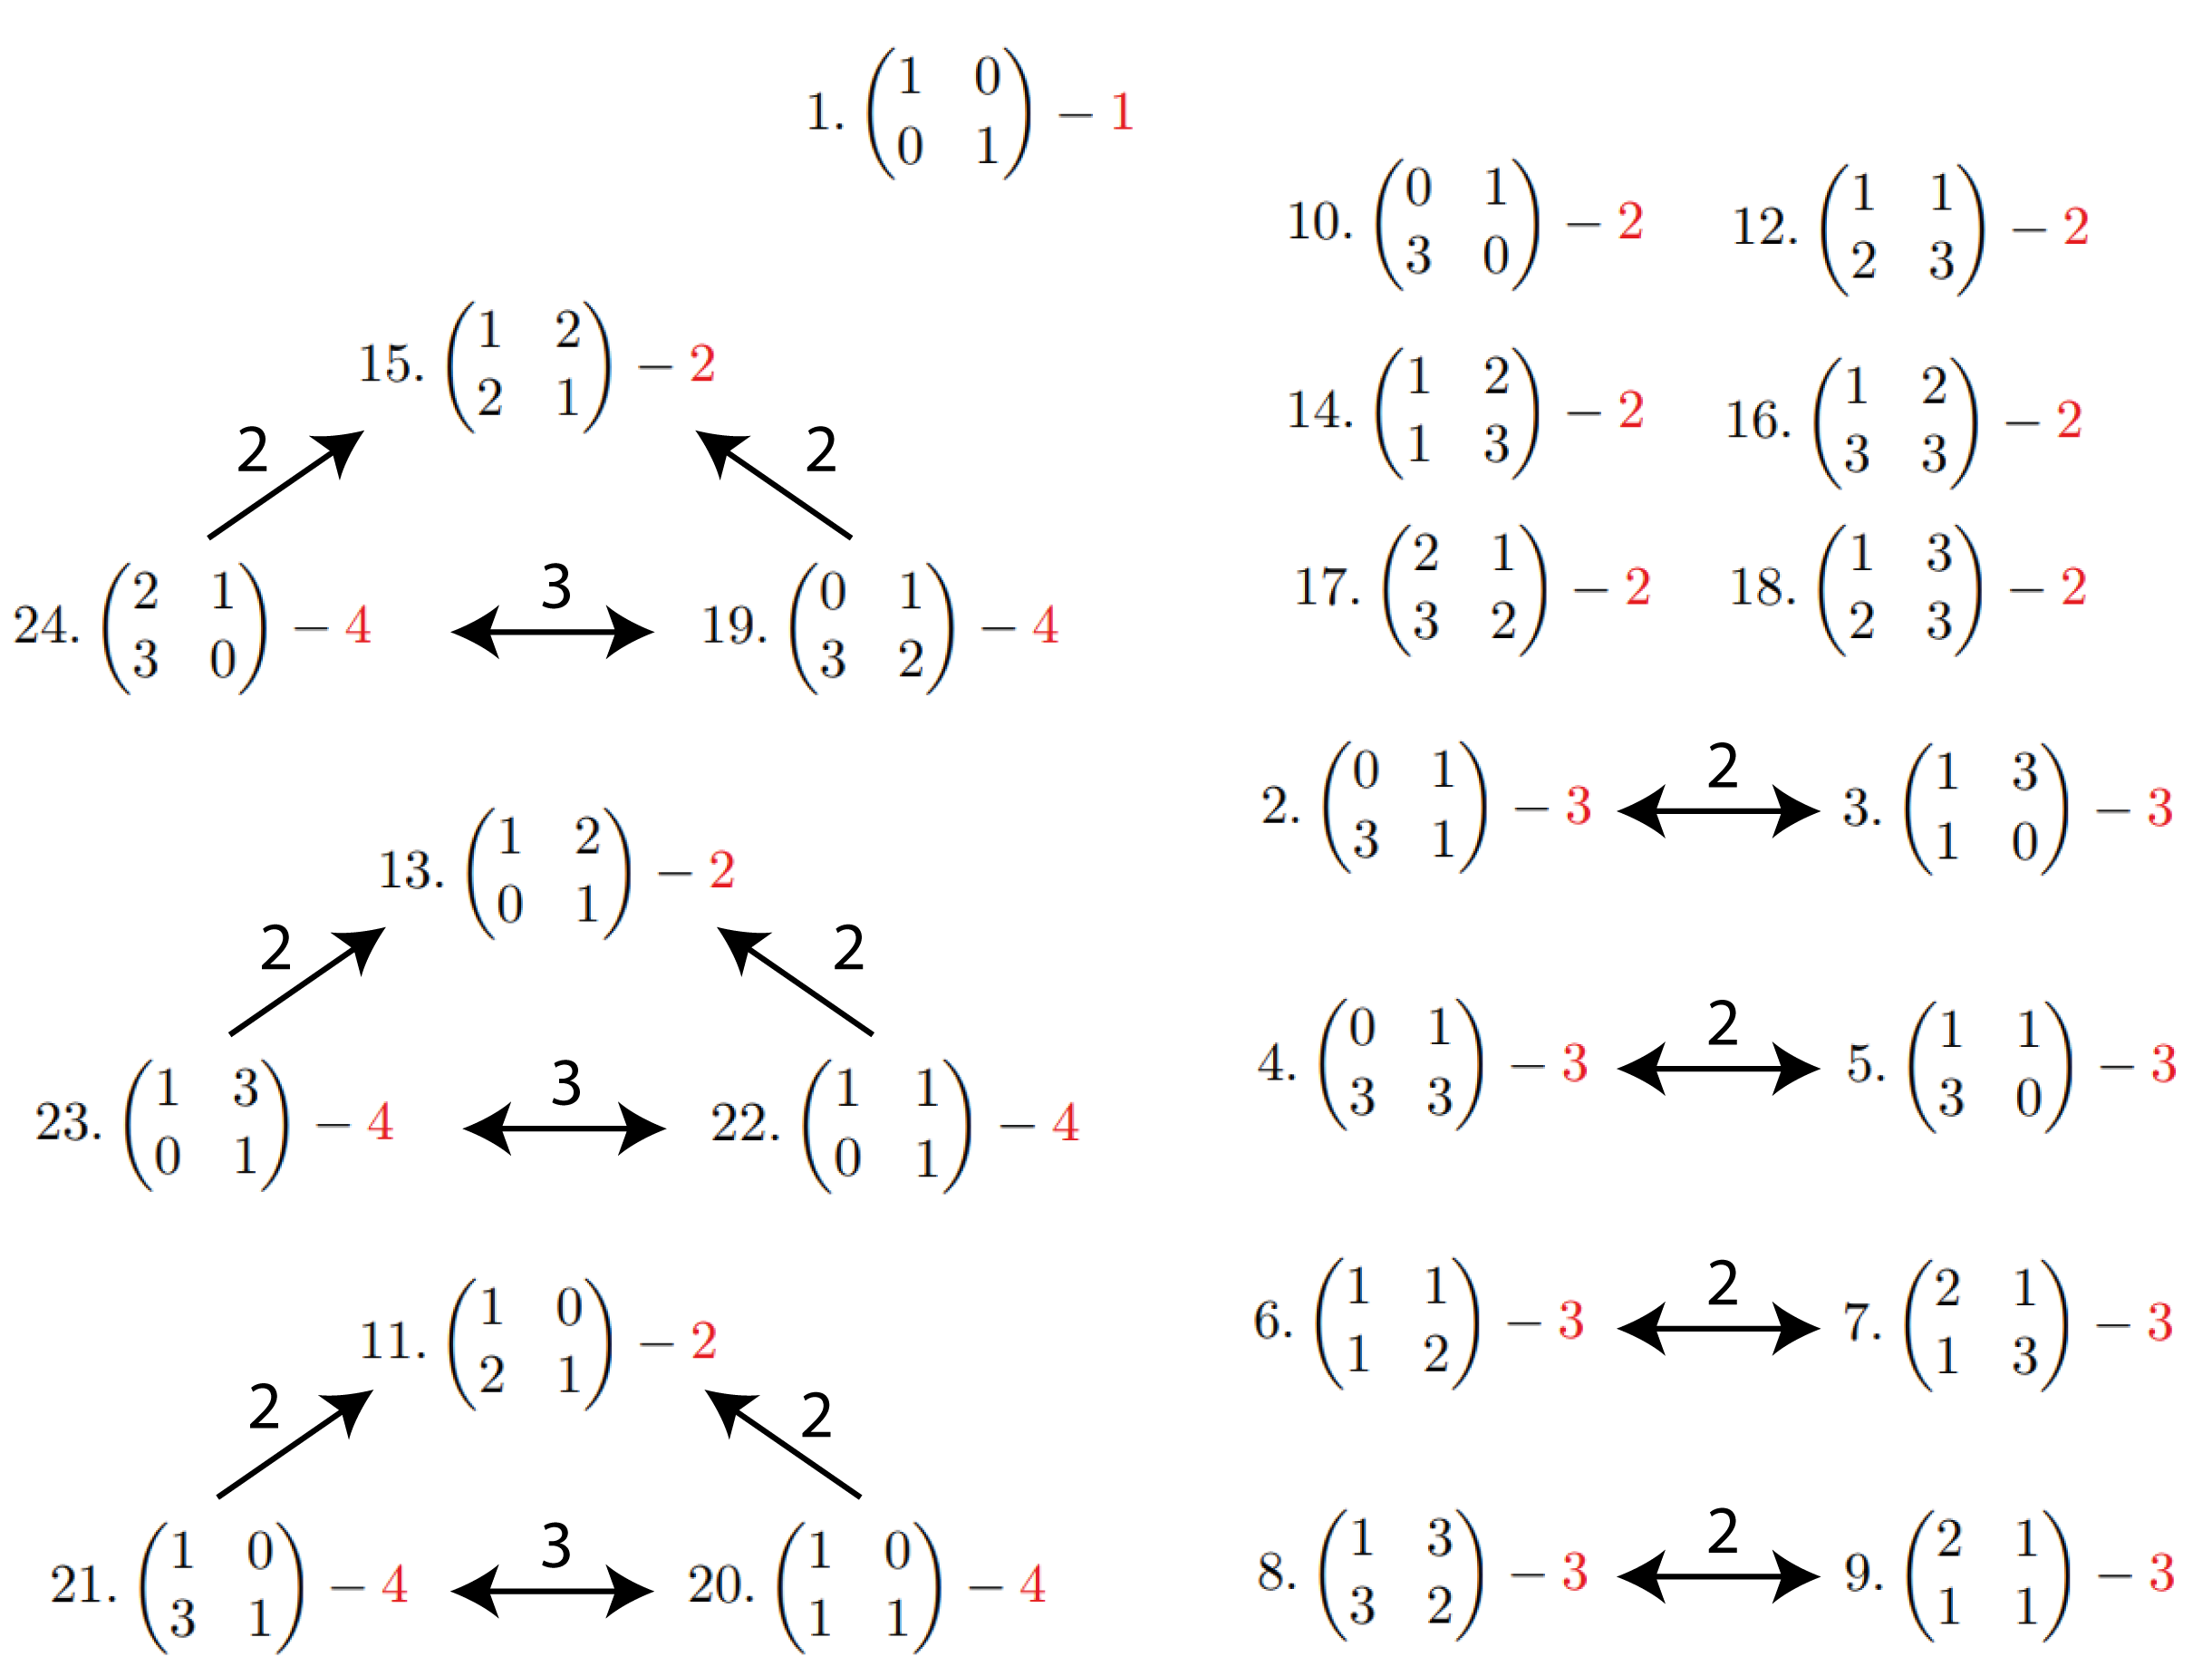
\includegraphics[width=13cm]{3_1.png}
      \end{figure}
      Подгруппы порядка 3:
      \[\left\{ \begin{pmatrix}
          1 & 0\\
          0 & 1
      \end{pmatrix},\ \begin{pmatrix}
          0 & 1\\
          3 & 1
      \end{pmatrix},\ \begin{pmatrix}
          1 & 3\\
          1 & 0
      \end{pmatrix}\right\}\]
      \[\left\{ \begin{pmatrix}
          1 & 0\\
          0 & 1
      \end{pmatrix},\ \begin{pmatrix}
          0 & 1\\
          3 & 3
      \end{pmatrix},\ \begin{pmatrix}
          1 & 1\\
          3 & 0
      \end{pmatrix}\right\}\]
      \[\left\{ \begin{pmatrix}
          1 & 0\\
          0 & 1
      \end{pmatrix},\ \begin{pmatrix}
          1 & 1\\
          1 & 2
      \end{pmatrix},\ \begin{pmatrix}
          2 & 1\\
          1 & 3
      \end{pmatrix}\right\}\]
      \[\left\{ \begin{pmatrix}
          1 & 0\\
          0 & 1
      \end{pmatrix},\ \begin{pmatrix}
          1 & 3\\
          3 & 2
      \end{pmatrix},\ \begin{pmatrix}
          2 & 1\\
          1 & 1
      \end{pmatrix}\right\}\]
      \[|H| = 4 \RA \left[ \begin{matrix}
          H \cong \Z_4 \text{ цикл}\\
          H \cong \Z_2 \times \Z_2
      \end{matrix}\right.\]
      Группы порядка 4 ($\cong \Z$):
      \[\left\{ \begin{pmatrix}
          1 & 0\\
          0 & 1
      \end{pmatrix},\ \begin{pmatrix}
          0 & 1\\
          3 & 2
      \end{pmatrix},\ \begin{pmatrix}
          1 & 2\\
          1 & 1
      \end{pmatrix},\ \begin{pmatrix}
          2 & 1\\
          3 & 0
      \end{pmatrix}\right\}\]
      \[\left\{ \begin{pmatrix}
          1 & 0\\
          0 & 1
      \end{pmatrix},\ \begin{pmatrix}
          1 & 2\\
          0 & 1
      \end{pmatrix},\ \begin{pmatrix}
          1 & 3\\
          0 & 1
      \end{pmatrix},\ \begin{pmatrix}
          1 & 1\\
          0 & 1
      \end{pmatrix}\right\}\]
      \[\left\{ \begin{pmatrix}
          1 & 0\\
          0 & 1
      \end{pmatrix},\ \begin{pmatrix}
          1 & 0\\
          1 & 1
      \end{pmatrix},\ \begin{pmatrix}
          1 & 0\\
          2 & 1
      \end{pmatrix},\ \begin{pmatrix}
          1 & 0\\
          3 & 1
      \end{pmatrix}\right\}\]
      \begin{figure}[H]
          \centering
          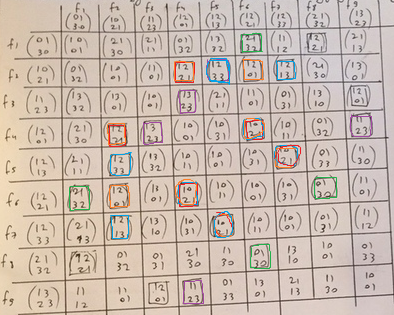
\includegraphics[width=10cm]{3_2.png}
      \end{figure}

      Группы порядка 4 ($\cong \Z_2 \times \Z_2$):
      \[\left\{ \begin{pmatrix}
          1 & 0\\
          0 & 1
      \end{pmatrix},\ \begin{pmatrix}
          1 & 2\\
          2 & 1
      \end{pmatrix},\ \begin{pmatrix}
          2 & 1\\
          3 & 2
      \end{pmatrix},\ \begin{pmatrix}
          0 & 1\\
          3 & 0
      \end{pmatrix}\right\}\]
      \[\left\{ \begin{pmatrix}
          1 & 0\\
          0 & 1
      \end{pmatrix},\ \begin{pmatrix}
          1 & 2\\
          0 & 1
      \end{pmatrix},\ \begin{pmatrix}
          1 & 2\\
          2 & 1
      \end{pmatrix},\ \begin{pmatrix}
          1 & 0\\
          2 & 1
      \end{pmatrix}\right\}\]
      \[\left\{ \begin{pmatrix}
          1 & 0\\
          0 & 1
      \end{pmatrix},\ \begin{pmatrix}
          1 & 0\\
          2 & 1
      \end{pmatrix},\ \begin{pmatrix}
          1 & 2\\
          1 & 3
      \end{pmatrix},\ \begin{pmatrix}
          1 & 2\\
          3 & 3
      \end{pmatrix}\right\}\]
      \[\left\{ \begin{pmatrix}
          1 & 0\\
          0 & 1
      \end{pmatrix},\ \begin{pmatrix}
          1 & 1\\
          2 & 3
      \end{pmatrix},\ \begin{pmatrix}
          1 & 2\\
          0 & 1
      \end{pmatrix},\ \begin{pmatrix}
          1 & 3\\
          2 & 3
      \end{pmatrix}\right\}\]

      \subsection{Второй пункт}
      \subsubsection{Формулировка}
      \item Выбрать одну из ненормальных подгрупп порядка 3 (если они есть) и выписать задаваемое ей разбиение $G$ на левые и правые классы смежности.

      В случае, если все подгруппы $G$ порядка 3 являются нормальными, найти нормальную подгруппу порядка 4 и выписать задаваемое ей разбиение $G$ на левые и правые классы смежности.
      \subsubsection{Вспомогательные факты}

      \begin{definition}
  		    $H<G$, тогда H - нормльная подгруппа, если $\forall h \in H,\ g \in G \Ra g^{-1}h g \in H$ - сопряжение элемента h с помощью элемента g, обозначается: $H \triangleleft G$
  		\end{definition}

      \subsubsection{Решение}
      Выберем одну из ненормальных подгрупп порядка 3:

      \[\text{Рассмотрим }\left\{ \begin{pmatrix}
          1 & 0\\
          0 & 1
      \end{pmatrix} ,\ \begin{pmatrix}
          0 & 1\\
          3 & 1
      \end{pmatrix},\ \begin{pmatrix}
          1 & 3\\
          1 & 0
      \end{pmatrix}\right\} = H \q \forall g \in G \q \forall h \in H \q g h g^{-1} \in H\]
      \[\text{Проверим: }\begin{pmatrix}
          0 & 1\\
          3 & 3
      \end{pmatrix} \begin{pmatrix}
          0 & 1\\
          3 & 1
      \end{pmatrix} \begin{pmatrix}
          1 & 1\\
          3 & 0
      \end{pmatrix} = \begin{pmatrix}
          1 & 3\\
          3 & 2
      \end{pmatrix} \begin{pmatrix}
          1 & 1\\
          3 & 0
      \end{pmatrix} = \begin{pmatrix}
          2 & 1\\
          1 & 3
      \end{pmatrix}\]
      $\Ra$ группа H - ненорм.

      Выпишем задаваемое H разбиение G на правые и левые классы смежности:

      То есть будем умножать элементы G на элементы H, выясняя, какие из них эквивалентны

      Правое (обозначение: черточка сверху - класс смежности):
      \[\ol{\begin{pmatrix}
          1 & 0\\
          0 & 1
      \end{pmatrix}} = \begin{pmatrix}
          1 & 0\\
          0 & 1
      \end{pmatrix} H = \left\{ \begin{pmatrix}
          1 & 0\\
          0 & 1
      \end{pmatrix},\ \begin{pmatrix}
          1 & 3\\
          3 & 2
      \end{pmatrix},\ \begin{pmatrix}
          2 & 1\\
          1 & 1
      \end{pmatrix} \right\} = \ol{\begin{pmatrix}
          1 & 3\\
          3 & 2
      \end{pmatrix}} = \ol{\begin{pmatrix}
          2 & 1\\
          1 & 1
      \end{pmatrix}}\]
      \[\ol{\begin{pmatrix}
          1 & 3\\
          1 & 0
      \end{pmatrix}} = \begin{pmatrix}
          1 & 3\\
          1 & 0
      \end{pmatrix} H = \left\{ \begin{pmatrix}
          1 & 3\\
          1 & 0
      \end{pmatrix},\ \begin{pmatrix}
          2 & 1\\
          1 & 3
      \end{pmatrix},\ \begin{pmatrix}
          1 & 0\\
          2 & 1
      \end{pmatrix} \right\} = \ol{\begin{pmatrix}
          2 & 1\\
          1 & 3
      \end{pmatrix}} = \ol{\begin{pmatrix}
          1 & 0\\
          2 & 1
      \end{pmatrix}}\]
      \[\ol{\begin{pmatrix}
          0 & 1\\
          3 & 3
      \end{pmatrix}} = \begin{pmatrix}
          0 & 1\\
          3 & 3
      \end{pmatrix} H = \left\{ \begin{pmatrix}
          0 & 1\\
          3 & 4
      \end{pmatrix},\ \begin{pmatrix}
          1 & 2\\
          0 & 1
      \end{pmatrix},\ \begin{pmatrix}
          1 & 1\\
          1 & 2
      \end{pmatrix} \right\} = \ol{\begin{pmatrix}
          1 & 2\\
          0 & 1
      \end{pmatrix}} = \ol{\begin{pmatrix}
          1 & 1\\
          1 & 2
      \end{pmatrix}}\]
      \[\ol{\begin{pmatrix}
          1 & 1\\
          3 & 0
      \end{pmatrix}} = \begin{pmatrix}
          1 & 1\\
          3 & 0
      \end{pmatrix} H = \left\{ \begin{pmatrix}
          1 & 1\\
          3 & 0
      \end{pmatrix},\ \begin{pmatrix}
          0 & 1\\
          3 & 1
      \end{pmatrix},\ \begin{pmatrix}
          1 & 2\\
          2 & 1
      \end{pmatrix} \right\} = \ol{\begin{pmatrix}
          0 & 1\\
          3 & 1
      \end{pmatrix}} = \ol{\begin{pmatrix}
          1 & 2\\
          2 & 1
      \end{pmatrix}}\]
      \[\ol{\begin{pmatrix}
          0 & 1\\
          3 & 0
      \end{pmatrix}} = \begin{pmatrix}
          0 & 1\\
          3 & 0
      \end{pmatrix} H = \left\{ \begin{pmatrix}
          0 & 1\\
          3 & 0
      \end{pmatrix},\ \begin{pmatrix}
          1 & 2\\
          1 & 3
      \end{pmatrix},\ \begin{pmatrix}
          1 & 1\\
          2 & 3
      \end{pmatrix} \right\} = \ol{\begin{pmatrix}
          1 & 2\\
          1 & 3
      \end{pmatrix}} = \ol{\begin{pmatrix}
          1 & 1\\
          2 & 3
      \end{pmatrix}}\]
      \[\ol{\begin{pmatrix}
          1 & 2\\
          3 & 3
      \end{pmatrix}} = \begin{pmatrix}
          1 & 2\\
          3 & 3
      \end{pmatrix} H = \left\{ \begin{pmatrix}
          1 & 2\\
          3 & 3
      \end{pmatrix},\ \begin{pmatrix}
          1 & 1\\
          0 & 1
      \end{pmatrix},\ \begin{pmatrix}
          0 & 1\\
          3 & 2
      \end{pmatrix} \right\} = \ol{\begin{pmatrix}
          1 & 1\\
          0 & 1
      \end{pmatrix}} = \ol{\begin{pmatrix}
          0 & 1\\
          3 & 2
      \end{pmatrix}}\]
      \[\ol{\begin{pmatrix}
          2 & 1\\
          3 & 2
      \end{pmatrix}} = \begin{pmatrix}
          2 & 1\\
          3 & 2
      \end{pmatrix} H = \left\{ \begin{pmatrix}
          2 & 1\\
          3 & 2
      \end{pmatrix},\ \begin{pmatrix}
          1 & 0\\
          1 & 1
      \end{pmatrix},\ \begin{pmatrix}
          1 & 3\\
          0 & 1
      \end{pmatrix} \right\} = \ol{\begin{pmatrix}
          1 & 0\\
          1 & 1
      \end{pmatrix}} = \ol{\begin{pmatrix}
          1 & 3\\
          0 & 1
      \end{pmatrix}}\]
      \[\ol{\begin{pmatrix}
          1 & 3\\
          2 & 3
      \end{pmatrix}} = \begin{pmatrix}
          1 & 3\\
          2 & 3
      \end{pmatrix} H = \left\{ \begin{pmatrix}
          1 & 3\\
          2 & 3
      \end{pmatrix},\ \begin{pmatrix}
          2 & 1\\
          3 & 0
      \end{pmatrix},\ \begin{pmatrix}
          1 & 0\\
          3 & 1
      \end{pmatrix} \right\} = \ol{\begin{pmatrix}
          2 & 1\\
          3 & 0
      \end{pmatrix}} = \ol{\begin{pmatrix}
          1 & 0\\
          3 & 1
      \end{pmatrix}}\]
      Левые:
      \[\ol{\begin{pmatrix}
          1 & 0\\
          0 & 1
      \end{pmatrix}} = \begin{pmatrix}
          1 & 0\\
          0 & 1
      \end{pmatrix} H = \left\{ \begin{pmatrix}
          1 & 0\\
          0 & 1
      \end{pmatrix},\ \begin{pmatrix}
          1 & 3\\
          3 & 2
      \end{pmatrix},\ \begin{pmatrix}
          2 & 1\\
          1 & 1
      \end{pmatrix} \right\} = \ol{\begin{pmatrix}
          1 & 3\\
          3 & 2
      \end{pmatrix}} = \ol{\begin{pmatrix}
          2 & 1\\
          1 & 1
      \end{pmatrix}}\]
      \[\ol{\begin{pmatrix}
          1 & 3\\
          1 & 0
      \end{pmatrix}} = \begin{pmatrix}
          1 & 3\\
          1 & 0
      \end{pmatrix} H = \left\{ \begin{pmatrix}
          1 & 3\\
          1 & 0
      \end{pmatrix},\ \begin{pmatrix}
          0 & 1\\
          3 & 3
      \end{pmatrix},\ \begin{pmatrix}
          1 & 2\\
          2 & 1
      \end{pmatrix} \right\} = \ol{\begin{pmatrix}
          0 & 1\\
          3 & 3
      \end{pmatrix}} = \ol{\begin{pmatrix}
          1 & 2\\
          2 & 1
      \end{pmatrix}}\]
      \[\ol{\begin{pmatrix}
          1 & 1\\
          3 & 0
      \end{pmatrix}} = \begin{pmatrix}
          1 & 1\\
          3 & 0
      \end{pmatrix} H = \left\{ \begin{pmatrix}
          1 & 1\\
          3 & 0
      \end{pmatrix},\ \begin{pmatrix}
          2 & 1\\
          1 & 3
      \end{pmatrix},\ \begin{pmatrix}
          1 & 2\\
          0 & 1
      \end{pmatrix} \right\} = \ol{\begin{pmatrix}
          2 & 1\\
          1 & 3
      \end{pmatrix}} = \ol{\begin{pmatrix}
          1 & 2\\
          0 & 1
      \end{pmatrix}}\]
      \[\ol{\begin{pmatrix}
          1 & 1\\
          1 & 2
      \end{pmatrix}} = \begin{pmatrix}
          1 & 1\\
          1 & 2
      \end{pmatrix} H = \left\{ \begin{pmatrix}
          1 & 1\\
          1 & 2
      \end{pmatrix},\ \begin{pmatrix}
          0 & 1\\
          3 & 1
      \end{pmatrix},\ \begin{pmatrix}
          1 & 0\\
          2 & 1
      \end{pmatrix} \right\} = \ol{\begin{pmatrix}
          0 & 1\\
          3 & 1
      \end{pmatrix}} = \ol{\begin{pmatrix}
          1 & 0\\
          2 & 1
      \end{pmatrix}}\]
      \[\ol{\begin{pmatrix}
          0 & 1\\
          3 & 0
      \end{pmatrix}} = \begin{pmatrix}
          0 & 1\\
          3 & 0
      \end{pmatrix} H = \left\{ \begin{pmatrix}
          0 & 1\\
          3 & 0
      \end{pmatrix},\ \begin{pmatrix}
          1 & 2\\
          1 & 3
      \end{pmatrix},\ \begin{pmatrix}
          1 & 1\\
          2 & 3
      \end{pmatrix} \right\} = \ol{\begin{pmatrix}
          1 & 1\\
          2 & 3
      \end{pmatrix}} = \ol{\begin{pmatrix}
          1 & 2\\
          1 & 3
      \end{pmatrix}}\]
      \[\ol{\begin{pmatrix}
          1 & 2\\
          3 & 3
      \end{pmatrix}} = \begin{pmatrix}
          1 & 2\\
          3 & 3
      \end{pmatrix} H = \left\{ \begin{pmatrix}
          1 & 2\\
          3 & 3
      \end{pmatrix},\ \begin{pmatrix}
          2 & 1\\
          3 & 0
      \end{pmatrix},\ \begin{pmatrix}
          1 & 3\\
          0 & 1
      \end{pmatrix} \right\} = \ol{\begin{pmatrix}
          2 & 1\\
          3 & 0
      \end{pmatrix}} = \ol{\begin{pmatrix}
          1 & 3\\
          0 & 1
      \end{pmatrix}}\]
      \[\ol{\begin{pmatrix}
          2 & 1\\
          3 & 2
      \end{pmatrix}} = \begin{pmatrix}
          2 & 1\\
          3 & 2
      \end{pmatrix} H = \left\{ \begin{pmatrix}
          2 & 1\\
          3 & 2
      \end{pmatrix},\ \begin{pmatrix}
          1 & 1\\
          0 & 1
      \end{pmatrix},\ \begin{pmatrix}
          1 & 0\\
          3 & 2
      \end{pmatrix} \right\} = \ol{\begin{pmatrix}
          1 & 1\\
          0 & 1
      \end{pmatrix}} = \ol{\begin{pmatrix}
          1 & 0\\
          3 & 2
      \end{pmatrix}}\]
      \[\ol{\begin{pmatrix}
          1 & 3\\
          2 & 3
      \end{pmatrix}} = \begin{pmatrix}
          1 & 3\\
          2 & 3
      \end{pmatrix} H = \left\{ \begin{pmatrix}
          1 & 3\\
          2 & 3
      \end{pmatrix},\ \begin{pmatrix}
          1 & 0\\
          1 & 1
      \end{pmatrix},\ \begin{pmatrix}
          0 & 1\\
          3 & 2
      \end{pmatrix} \right\} = \ol{\begin{pmatrix}
          1 & 0\\
          1 & 1
      \end{pmatrix}} = \ol{\begin{pmatrix}
          0 & 1\\
          3 & 2
      \end{pmatrix}}\]
      \subsection{Третий пункт}
      \subsubsection{Формулировка}
      \item Выбрать одну из нормальных подгрупп $G$ порядка 3 (если они есть),
      построить таблицу Кэли для соответствующей факторгруппы и определить, какой из перечисленных в приложении групп порядка 8 она изоморфна.

      В случае, если все подгруппы $G$ порядка 3 являются ненормальными,
      найти нормальную подгруппу порядка 2, построить таблицу Кэли для
      соответствующей факторгруппы и определить, какой из перечисленных в приложении групп порядка 12 она изоморфна.

      В случае, если все подгруппы $G$ порядка 2 и 3 являются ненормальными, найти нормальную подгруппу порядка 4 и построить таблицу Кэли для соответствующей факторгруппы. Кроме того, в этом случае
      необходимо выбрать произвольную подгруппу G порядка 8 и определить, какой из перечисленных в приложении групп она изоморфна.
      \subsubsection{Вспомогательные факты}
      \begin{utv}
          Классы эквивалентности либо совпадают, либо не пересекаются
      \end{utv}
      \subsubsection{Решение}
      Решение: выберем одну из нормальных подгрупп G:\\
      Порядка 3:\\
      \[\text{Рассмотрим } \left\{ \begin{pmatrix}
          1 & 0\\
          0 & 1
      \end{pmatrix},\ \begin{pmatrix}
          0 & 1\\
          3 & 3
      \end{pmatrix},\ \begin{pmatrix}
          1 & 1\\
          3 & 0
      \end{pmatrix}\right\}=H\]
      \[\begin{pmatrix}
          0 & 1\\
          3 & 1
      \end{pmatrix} \begin{pmatrix}
          0 & 1\\
          3 & 3
      \end{pmatrix} \begin{pmatrix}
          1 & 3\\
          1 & 0
      \end{pmatrix} = \begin{pmatrix}
          1 & 1\\
          1 & 2
      \end{pmatrix} \begin{pmatrix}
          1 & 3\\
          1 & 0
      \end{pmatrix} = \begin{pmatrix}
          2 & 1\\
          1 & 1
      \end{pmatrix} \not \in H \RA \text{ненорм.}\]
      \[\text{Рассмотрим } \left\{ \begin{pmatrix}
          1 & 0\\
          0 & 1
      \end{pmatrix},\ \begin{pmatrix}
          1 & 1\\
          1 & 2
      \end{pmatrix},\ \begin{pmatrix}
          2 & 1\\
          1 & 3
      \end{pmatrix}\right\}=H\]
      \[\begin{pmatrix}
          1 & 3\\
          1 & 0
      \end{pmatrix} \begin{pmatrix}
          1 & 1\\
          1 & 2
      \end{pmatrix} \begin{pmatrix}
          0 & 1\\
          3 & 1
      \end{pmatrix} = \begin{pmatrix}
          0 & 3\\
          1 & 1
      \end{pmatrix} \begin{pmatrix}
          0 & 1\\
          3 & 1
      \end{pmatrix} = \begin{pmatrix}
          1 & 3\\
          3 & 2
      \end{pmatrix} \not \in H \RA \text{ненорм.}\]
      \[\text{Рассмотрим } \left\{ \begin{pmatrix}
          1 & 0\\
          0 & 1
      \end{pmatrix},\ \begin{pmatrix}
          1 & 3\\
          3 & 2
      \end{pmatrix},\ \begin{pmatrix}
          2 & 1\\
          1 & 1
      \end{pmatrix}\right\}=H\]
      \[\begin{pmatrix}
          0 & 1\\
          3 & 1
      \end{pmatrix} \begin{pmatrix}
          1 & 3\\
          3 & 2
      \end{pmatrix} \begin{pmatrix}
          1 & 3\\
          1 & 0
      \end{pmatrix} = \begin{pmatrix}
          1 & 2\\
          2 & 1
      \end{pmatrix} \begin{pmatrix}
          1 & 3\\
          1 & 0
      \end{pmatrix} = \begin{pmatrix}
          1 & 1\\
          1 & 2
      \end{pmatrix} \not \in H \RA \text{ненорм.}\]
      Т.о. все группы порядка 3 ненорм.\\ \ \\
      Порядка 2:

      Нет: среди подгрупп порядка 2 нет нормальных, т.к. нет ни одного элемента порядка 2, который коммутировал бы со всеми (см. табл. Кэли)\\ \ \\
      Порядка 4:
      \[\left\{\begin{pmatrix}
          1 & 0\\
          0 & 1
      \end{pmatrix},\ \begin{pmatrix}
          1 & 2\\
          2 & 1
      \end{pmatrix},\ \begin{pmatrix}
          1 & 0\\
          2 & 1
      \end{pmatrix},\ \begin{pmatrix}
          1 & 2\\
          0 & 1
      \end{pmatrix}\right\}\]
      \begin{tabular}{c|c}
        $\begin{pmatrix}
            1 & 0\\
            0 & 1
        \end{pmatrix} H$ & $H \begin{pmatrix}
            1 & 0\\
            0 & 1
        \end{pmatrix}$\\
        \hline
        $\begin{pmatrix}
            1 & 0\\
            0 & 1
        \end{pmatrix}$ & $\begin{pmatrix}
            1 & 0\\
            0 & 1
        \end{pmatrix}$\\
        $\begin{pmatrix}
            1 & 2\\
            2 & 1
        \end{pmatrix}$ & $\begin{pmatrix}
            1 & 2\\
            2 & 1
        \end{pmatrix}$\\
        $\begin{pmatrix}
            1 & 0\\
            2 & 1
        \end{pmatrix}$ & $\begin{pmatrix}
            1 & 0\\
            2 & 1
        \end{pmatrix}$\\
        $\begin{pmatrix}
            1 & 2\\
            0 & 1
        \end{pmatrix}$ & $\begin{pmatrix}
            1 & 2\\
            0 & 1
        \end{pmatrix}$
      \end{tabular}
      \begin{tabular}{c|c}
        $\begin{pmatrix}
            0 & 1\\
            3 & 1
        \end{pmatrix} H$ & $H \begin{pmatrix}
            0 & 1\\
            3 & 1
        \end{pmatrix}$\\
        \hline
        $\begin{pmatrix}
            0 & 1\\
            3 & 1
        \end{pmatrix}$ & $\begin{pmatrix}
            0 & 1\\
            3 & 1
        \end{pmatrix}$\\
        $\begin{pmatrix}
            2 & 1\\
            1 & 3
        \end{pmatrix}$ & $\begin{pmatrix}
            2 & 1\\
            1 & 1
        \end{pmatrix}$\\
        $\begin{pmatrix}
            2 & 1\\
            1 & 1
        \end{pmatrix}$ & $\begin{pmatrix}
            0 & 1\\
            3 & 3
        \end{pmatrix}$\\
        $\begin{pmatrix}
            0 & 1\\
            3 & 3
        \end{pmatrix}$ & $\begin{pmatrix}
            2 & 1\\
            1 & 3
        \end{pmatrix}$
      \end{tabular}
      \begin{tabular}{c|c}
        $\begin{pmatrix}
            1 & 3\\
            1 & 0
        \end{pmatrix} H$ & $H \begin{pmatrix}
            1 & 3\\
            1 & 0
        \end{pmatrix}$\\
        \hline
        $\begin{pmatrix}
            1 & 3\\
            1 & 0
        \end{pmatrix}$ & $\begin{pmatrix}
            1 & 3\\
            1 & 0
        \end{pmatrix}$\\
        $\begin{pmatrix}
            1 & 3\\
            3 & 2
        \end{pmatrix}$ & $\begin{pmatrix}
            1 & 1\\
            1 & 2
        \end{pmatrix}$\\
        $\begin{pmatrix}
            1 & 1\\
            3 & 0
        \end{pmatrix}$ & $\begin{pmatrix}
            1 & 3\\
            3 & 2
        \end{pmatrix}$\\
        $\begin{pmatrix}
            1 & 1\\
            1 & 2
        \end{pmatrix}$ & $\begin{pmatrix}
            1 & 1\\
            3 & 0
        \end{pmatrix}$
      \end{tabular}
      \begin{tabular}{c|c}
        $\begin{pmatrix}
            0 & 1\\
            3 & 0
        \end{pmatrix} H$ & $H \begin{pmatrix}
            0 & 1\\
            3 & 0
        \end{pmatrix}$\\
        \hline
        $\begin{pmatrix}
            0 & 1\\
            3 & 0
        \end{pmatrix}$ & $\begin{pmatrix}
            0 & 1\\
            3 & 0
        \end{pmatrix}$\\
        $\begin{pmatrix}
            2 & 1\\
            3 & 2
        \end{pmatrix}$ & $\begin{pmatrix}
            2 & 1\\
            3 & 2
        \end{pmatrix}$\\
        $\begin{pmatrix}
            2 & 1\\
            3 & 0
        \end{pmatrix}$ & $\begin{pmatrix}
            0 & 1\\
            3 & 2
        \end{pmatrix}$\\
        $\begin{pmatrix}
            0 & 1\\
            3 & 2
        \end{pmatrix}$ & $\begin{pmatrix}
            2 & 1\\
            3 & 0
        \end{pmatrix}$
      \end{tabular}
      \begin{tabular}{c|c}
        $\begin{pmatrix}
            1 & 1\\
            2 & 3
        \end{pmatrix} H$ & $H \begin{pmatrix}
            1 & 1\\
            2 & 3
        \end{pmatrix}$\\
        \hline
        $\begin{pmatrix}
            1 & 1\\
            2 & 3
        \end{pmatrix}$ & $\begin{pmatrix}
            1 & 1\\
            2 & 3
        \end{pmatrix}$\\
        $\begin{pmatrix}
            1 & 1\\
            0 & 1
        \end{pmatrix}$ & $\begin{pmatrix}
            1 & 3\\
            0 & 1
        \end{pmatrix}$\\
        $\begin{pmatrix}
            1 & 3\\
            0 & 1
        \end{pmatrix}$ & $\begin{pmatrix}
            1 & 1\\
            0 & 1
        \end{pmatrix}$\\
        $\begin{pmatrix}
            1 & 3\\
            2 & 3
        \end{pmatrix}$ & $\begin{pmatrix}
            1 & 3\\
            2 & 3
        \end{pmatrix}$
      \end{tabular}
      \begin{tabular}{c|c}
        $\begin{pmatrix}
            1 & 2\\
            3 & 3
        \end{pmatrix} H$ & $H \begin{pmatrix}
            1 & 2\\
            3 & 3
        \end{pmatrix}$\\
        \hline
        $\begin{pmatrix}
            1 & 2\\
            3 & 3
        \end{pmatrix}$ & $\begin{pmatrix}
            1 & 2\\
            3 & 3
        \end{pmatrix}$\\
        $\begin{pmatrix}
            1 & 0\\
            1 & 1
        \end{pmatrix}$ & $\begin{pmatrix}
            1 & 0\\
            3 & 1
        \end{pmatrix}$\\
        $\begin{pmatrix}
            1 & 2\\
            1 & 3
        \end{pmatrix}$ & $\begin{pmatrix}
            1 & 2\\
            1 & 3
        \end{pmatrix}$\\
        $\begin{pmatrix}
            1 & 0\\
            3 & 1
        \end{pmatrix}$ & $\begin{pmatrix}
            1 & 0\\
            1 & 1
        \end{pmatrix}$
      \end{tabular}
      Разбилось на 24 элемента, значит других элементов факторгруппы нет

      Построим таблицу Кэли для факторгруппы $G/H$:
      \begin{figure}[h]
          \centering
          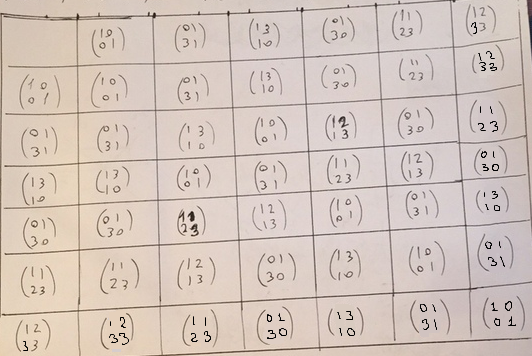
\includegraphics[width=10cm]{3_3.png}
      \end{figure}
      \[\text{Пример: } \begin{pmatrix}
          1 & 3\\
          1 & 0
      \end{pmatrix} \cdot \begin{pmatrix}
          1 & 2\\
          3 & 3
      \end{pmatrix} = \begin{pmatrix}
          10 & 11\\
          1 & 2
      \end{pmatrix} = \begin{pmatrix}
          2 & 1\\
          3 & 2
      \end{pmatrix} \sim \begin{pmatrix}
          0 & 1\\
          3 & 0
      \end{pmatrix}\]

      \subsection{Четвертый пункт}
      \subsubsection{Формулировка}
      \item Описать явно изоморфизм между соответствующими группами из предыдущего пункта и доказать, что это изоморфизм. (В случае представления совпадающий таблиц Кэли необходимо продемонстрировать, каким образом происходил поиск соответствующего упорядочивания).
      \subsubsection{Вспомогательные факты}
      \subsubsection{Решение}
      \subsection{Пятый пункт}
      \subsubsection{Формулировка}
      \item Есть ли изоморфная $G$ группа среди трех следующих за ней по списку?
      \subsubsection{Вспомогательные факты}
      \subsubsection{Решение}
      \subsection{Шестой пункт}
      \subsubsection{Формулировка}
      \item Найти коммутант $G$.
      \subsubsection{Вспомогательные факты}
      \subsubsection{Решение}
    \end{enumerate}
\end{document}
